\chapter{Conclusion} \label{chapter:conclusion}
\glsresetall


\section{Summary}

The widespread adoption of \gls{ml} in safety-critical \glspl{cps} has reshaped the way we create and deploy intelligent control systems. Whether it is autonomous vehicles navigating busy city streets or medical devices tracking patient vitals, \gls{ml}-driven solutions are now making high-stakes decisions that directly affect human lives. At the same time, this shift has exposed new hurdles—traditional, monolithic \gls{ml} models were not built with rigorous verification, precise timing analysis, strong safety guarantees, or clear explainability in mind. Balancing the intricate demands of these systems against the "black-box" nature of deep neural networks presents a significant challenge: we want the speed and accuracy \gls{ml} offers, but we cannot sacrifice the safety that critical applications require.

In this thesis, we tackle that challenge head-on by proposing a compositional \gls{ml} paradigm tailored for \gls{cps}. Instead of using an \gls{ml} model as one large block, we break it down into smaller sub-models, with similar functional behaviour, that can be independently analysed and then composed back together. This modular approach preserves the original network's behaviour while giving us the tools to verify timing properties, construct safer models by design, and offer better explanations for each component's decisions. By weaving compositionality into the very fabric of \gls{ml}-based \glspl{cps}, we lay the groundwork for systems that are not only powerful but also provably safe, time-predictable, and inherently interpretable. The contributions of this thesis are summarised as follows:

\begin{enumerate}
    \item \textbf{Compositional Model Development and Hardware Implementation (Chapter 3):} We introduced the formation of compositional ANN models using a systematic decomposition of monolithic ANN models into smaller, functionally equivalent sub-models. We demonstrated this methodology across multiple real-world datasets, including transportation data for autonomous vehicle lane-changing and depressive mood score prediction, showing that compositional designs can achieve significant reductions in hardware footprint (up to 53\% reduction in resources) and computational complexity (up to 40\% reduction in computations) while maintaining comparable performance to monolithic approaches.

 It is also here that we developed novel compilation frameworks that translate Python-based ANN models to both \glspl{vhdl} (for \gls{fpga} implementation) and C code (for embedded systems), enabling formal \gls{wcet} analysis. Our compilers specifically support the compositional architecture proposed in this work, addressing a critical gap in existing tools that cannot handle compositional ML designs with ANNs. We demonstrated that compositional models can achieve up to 85\% reduction in \gls{wcet} compared to monolithic implementations, making them suitable for real-time applications with strict timing constraints.

    \item \textbf{Safe-by-Construction Design (Chapter 4):} We introduced a policy-driven framework for building safe-by-construction ML-based CPSs that addresses the fundamental challenge of ensuring safety in data-driven approaches. Using an autonomous vehicle as a case study, we demonstrated how safety properties (described as \gls{vdta}) can be mined from real-world data and used to guide the design and training of compositional models of various kinds (e.g. \glspl{ann}, \glspl{svm}, etc.). We show how our training approach reduces the number of unsafe scenarios. Our \gls{re} mechanism monitors policy-trained model outputs in real-time and ensures policy adherence, providing a fail-safe for unexpected scenarios where learned models may fail to comply with safety expectations. This approach bridges the gap between formal verification and \gls{ml}, enabling the development of systems that are both performant and provably safe.
    
    \item \textbf{Explainable ML Models (Chapter 5):} We developed a novel explainability paradigm for both monolithic and compositional \gls{ml} models that addresses the critical need for explainability in safety-critical applications (e.g. medical devices) using \gls{ml} models. Our approach combines multiple explainability techniques—\glspl{shap}, \glspl{ale}, and Anchors—to provide actionable insights at both the sub-model and system levels. Using a personalised depression prediction case study, we demonstrated how compositional models can offer enhanced explainability by providing more detailed explanations compared to monolithic approaches, enabling healthcare professionals to better understand how different factors contribute to patient outcomes and make informed intervention decisions. 
    
\end{enumerate}

Throughout the thesis, we validated our compositional framework through comprehensive case studies in two critical domains: autonomous vehicles and healthcare. These case studies demonstrate the practical applicability of our approach and provide concrete evidence of its benefits in terms of performance, safety, and explainability. The results show that compositional \gls{ml} can address the fundamental limitations of current approaches while maintaining (and in some cases enhancing) the performance benefits that make \gls{ml} attractive for \gls{cps} applications.

The implications of this work extend beyond the specific applications considered in this thesis. The compositional framework we have developed provides a general methodology that can be applied to any domain where \gls{ml} systems must meet rigorous safety, timing, and explainability requirements. As \gls{ml} continues to permeate safety-critical applications—from medical devices and autonomous vehicles to industrial control systems and aerospace applications—the need for compositional approaches will only grow more urgent.

\begin{figure}[htbp]
    \centering
    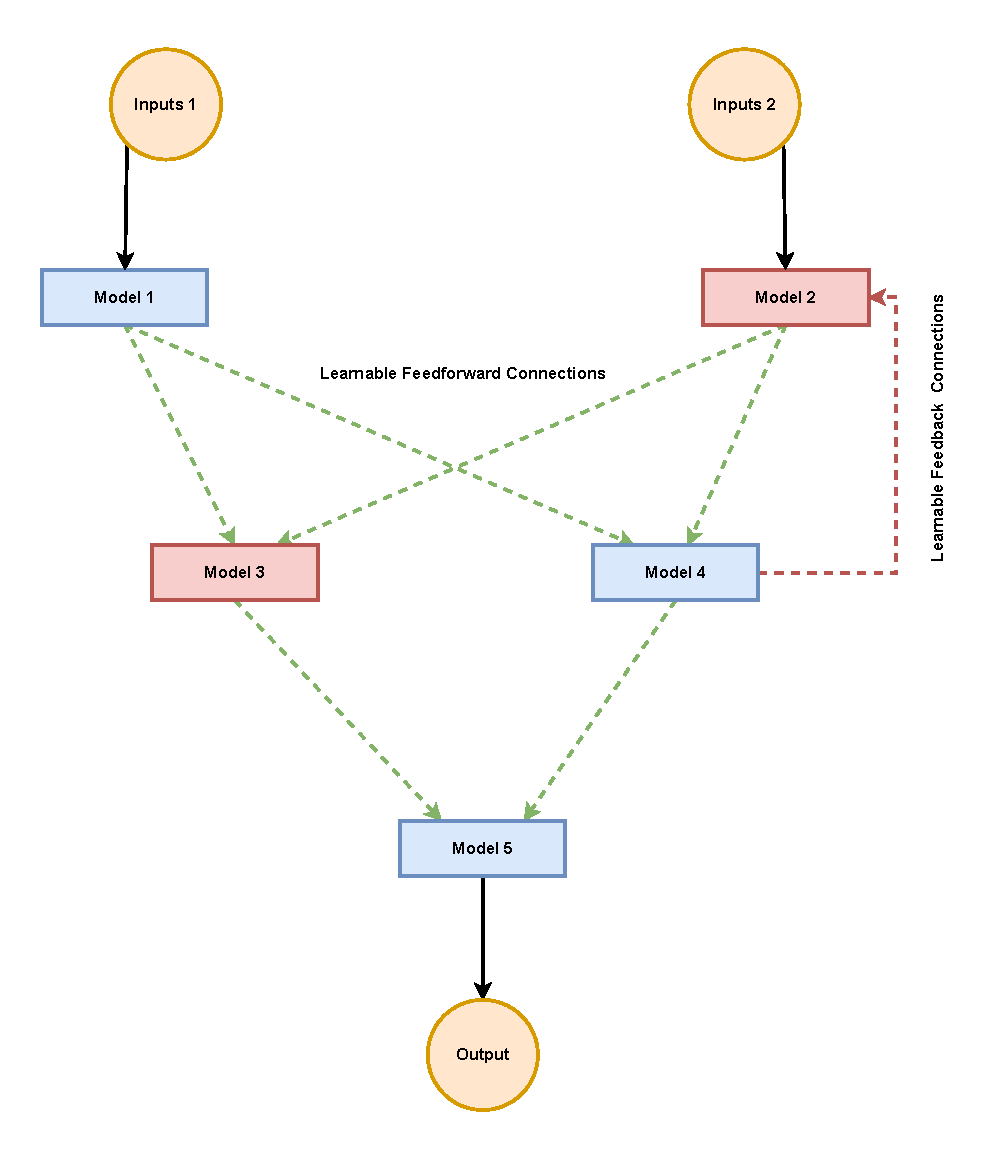
\includegraphics[width=0.8\textwidth]{conclusions/fig/future_work_1.pdf}
    \caption{An updated compositional architecture for \gls{ml}-based \glspl{cps} with inter-model connections that are learnt and not statically defined. The architecture is also composed of models of multiple types (red and blue boxes) that are combined in a hierarchical manner, as well as feedback loops.}
    \label{fig:future_work_1}
\end{figure}

\section{Limitations and Future Directions}

Despite the significant progress made in this thesis, several limitations remain that open up promising directions for future research in compositional \gls{ml} for cyber-physical systems:

\begin{enumerate}
    \item \textbf{Advanced Compositional Models and Architectures:}
    \begin{itemize}
        \item We have only considered the use of MLP-based models in a feedforward connection in our case studies. Future work could explore the use of more sophisticated compositional patterns beyond the simple parallel and sequential compositions considered in this thesis. This includes feedback loops and dynamic compositions that can adapt their structure based on runtime conditions (see Figure \ref{fig:future_work_1}). Furthermore, the use of more sophisticated models (e.g. \glspl{cnn}, \glspl{rnn}, etc.) is an important direction for future work as it will allow us to handle more complex data and tasks.
        
        \begin{figure}[htbp]
            \centering
            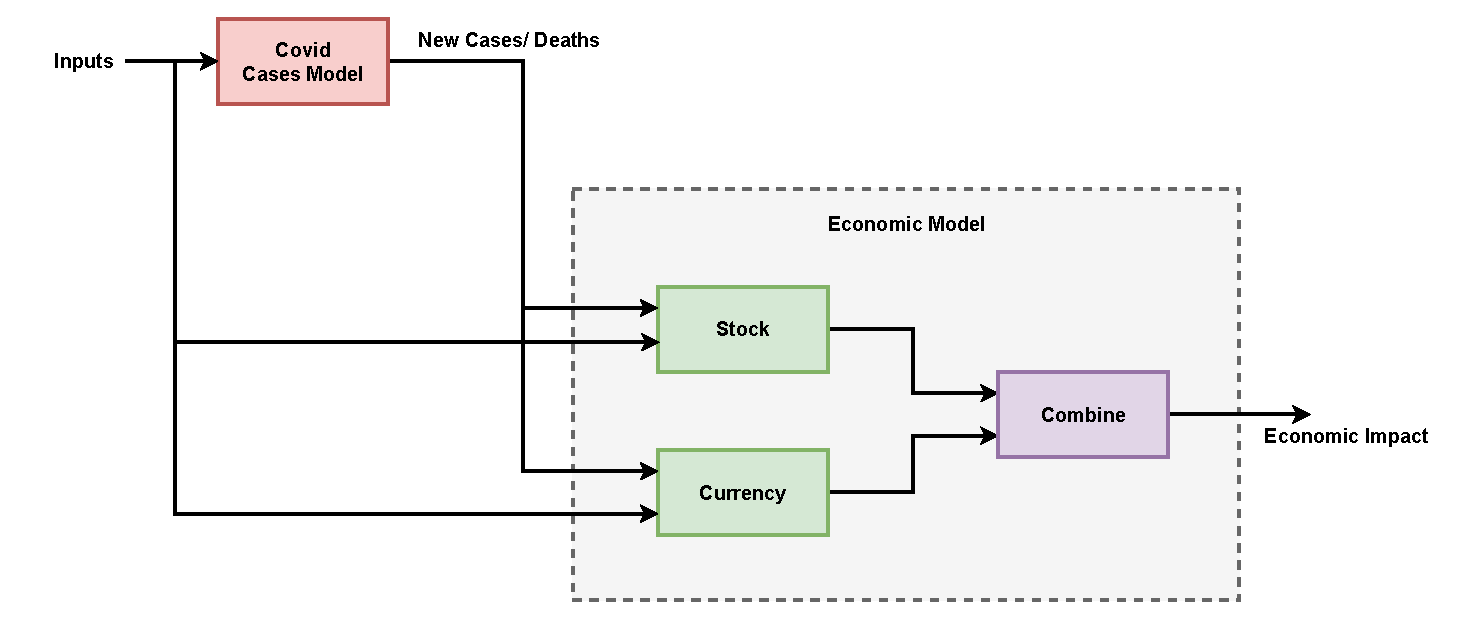
\includegraphics[width=\textwidth]{conclusions/fig/Covid19.pdf}
            \caption{Compositional model for Covid-19 Economic Impact Prediction.}
            \label{fig:covid19}
        \end{figure}
        
        \item We would also like to test the applicability of our compositional framework to more case studies, like the one shown in Figure \ref{fig:covid19}, where we could use the compositional framework to predict the economic impact of the Covid-19 pandemic. We use a model to predict the number of cases and deaths and pass this into Stock and Currency models (with other inputs) to predict the economic impact. This compositional design separates concerns and makes the decision flow more apparent.

        \item While we focused on manual decomposition of monolithic models, either from a domain expert or a pre-defined policy structure, future work could explore automated methods for learning optimal compositional structures from data. This could include \gls{rl} approaches that discover compositions that optimise for performance, safety, and explainability simultaneously.
        
        \item We have only considered small to medium-sized \glspl{ann} in our case studies. Future work could explore the use of larger \glspl{ann} (e.g. \glspl{llm}) and their compositional architectures, especially in the context of \glspl{cps} that require high-performance and low-latency.
    \end{itemize}


\begin{figure}[htbp]
    \centering
    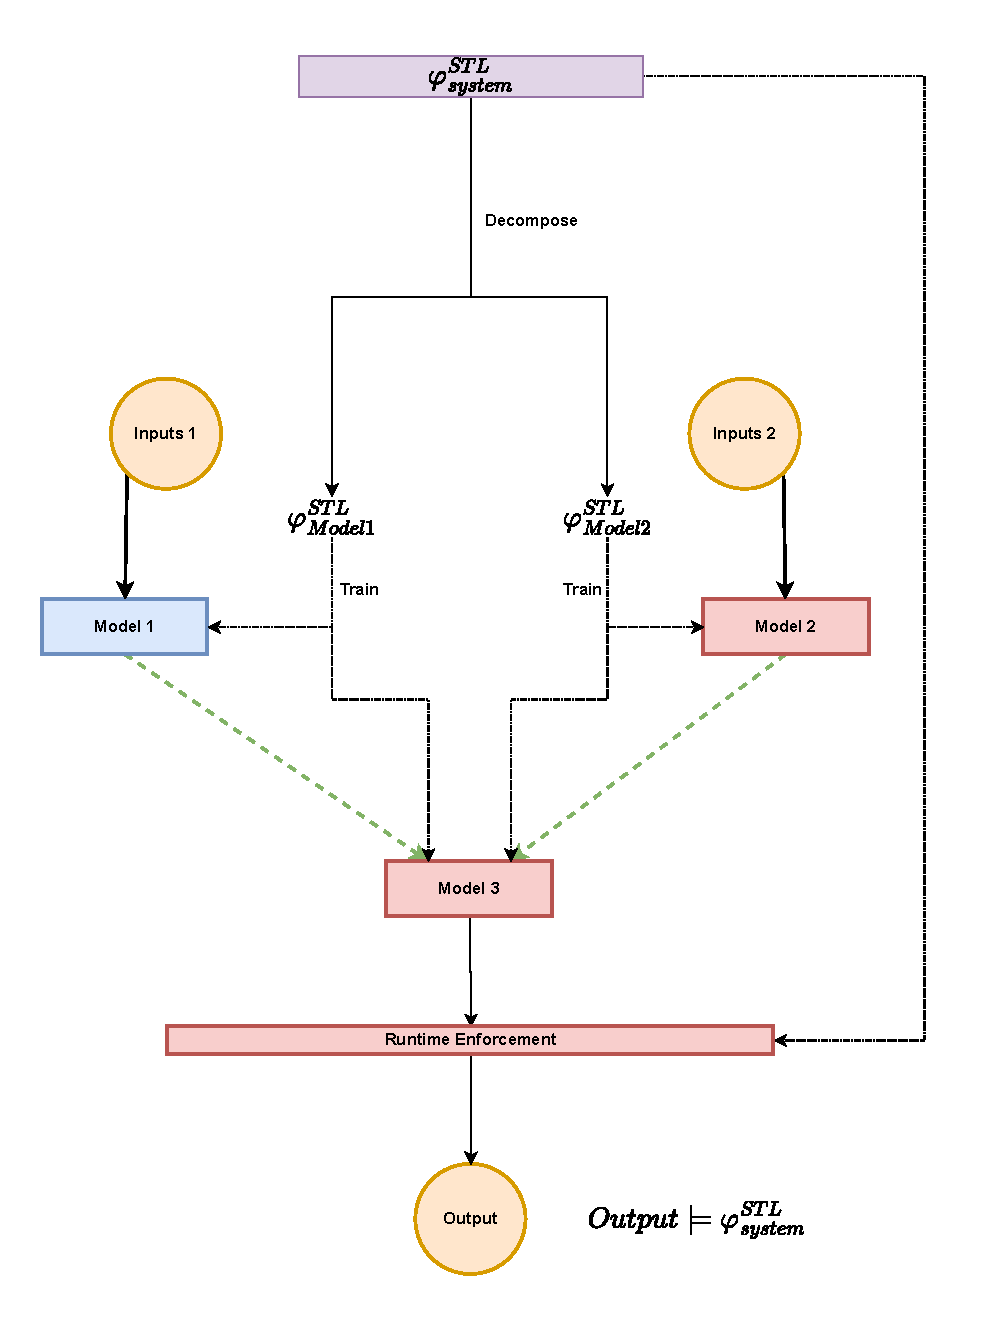
\includegraphics[width=\textwidth]{conclusions/fig/future_work_2.pdf}
    \caption{Updating the compositional training framework to \gls{stl} specifications. The system-level specification is decomposed into sub-model specifications and used to guide the training of the compositional models and the runtime enforcement of the compositional models. The decomposition is done so that the sub-model specifications are not contradictory and the system-level specification is satisfied.}
    \label{fig:future_work_2}
\end{figure}

    \item \textbf{Integration with Formal Temporal Specifications:} Our work establishes the theoretical foundation for compositional policy-based training of \gls{ml}-based \glspl{cps} and their runtime enforcement, but we do not use temporal specifications, which are frequently used to specify safety properties of \glspl{cps}. Future work could explore the integration of temporal specifications (such as \gls{ltl} \cite{de_giacomo_linear_2013_ltl}, \gls{ctl} \cite{vardi_branching_2001_ctl} and \gls{stl} \cite{donze_on_2013_stl}) to specify safety properties of \glspl{cps} and use them to guide the training of compositional models. The training will be challenging as a new methodology will have to be developed to handle the temporal specifications, which span multiple time-steps. The runtime enforcement toolchain we used \footnote{https://github.com/PRETgroup/easy-rte} will have to be updated to handle the temporal specifications, especially for \gls{stl} specifications (see Figure \ref{fig:future_work_2} for an example modelling flow).
    
    \item \textbf{Scalability Analysis:} The scalability (time and memory) of the compositional methodologies described have not been formally tested with larger networks and datasets. Future work could explore the scalability of the compositional methodologies described in this thesis.
    
    
    \item \textbf{Standardisation and Tooling:} As compositional approaches gain adoption, there will be a need for standardised interfaces, tools, and methodologies. Although we have developed a compiler for \glspl{vhdl} and C code, a framework for policy-based training of \gls{ml}-based \glspl{cps}, and a compositional explainability framework, we have not developed the interfaces to make them easily usable by practitioners across different domains. Future work could focus on developing open-source frameworks and tools that make compositional \gls{ml} accessible to practitioners across different domains. Also, the toolchain will have to be updated to handle the feedback loops in the compositional models and any addition of new types of models.
    
    \item \textbf{Enhancing Compositional Explainability:} Our compositional explainability framework is a novel approach to explainability that combines compositionality with multiple post-hoc explainability techniques. However, it requires the manual analysis of plots and conditionals, which may reduce its utility for non-domain experts. Developing a framework that provides explanations in a more accessible format (e.g. natural language) is an important direction for future work. Also, experimentation with other ML models, explainability techniques, and the inclusion of explanations that comment on causal relationships are important directions for future work.

\end{enumerate}

\section{Final Remarks}

The integration of \gls{ml} into safety-critical cyber-physical systems represents one of the most significant technological challenges of our time. While ML offers unprecedented capabilities for handling complex, nonlinear relationships in real-world systems, its black-box nature and lack of formal guarantees create fundamental barriers to adoption in safety-critical domains. This thesis demonstrates that compositionality provides a structured solution to these challenges, enabling the development of ML systems that are not only more performant but also more time-analysable, implementable, safer, and trustworthy than their monolithic counterparts.

The compositional framework we have developed represents a significant shift in how we think about \gls{ml} for safety-critical applications. Rather than treating ML models as black boxes that must be wrapped with safety mechanisms, our approach embeds safety, verification, and explainability into the very structure of the models themselves. This fundamental change in perspective opens new possibilities for deploying ML in domains where reliability and trust are paramount.

As we move toward an increasingly automated and intelligent world, the principles and methodologies developed in this thesis will become essential for ensuring that the benefits of \gls{ml} can be safely and reliably deployed in applications that directly impact human safety and well-being. While significant challenges remain in extension of the compositional framework, the foundation we have established provides a clear path forward for developing ML systems that can meet the rigorous requirements of safety-critical applications while delivering the performance benefits that make \gls{ml} so valuable. The future of safe, reliable, and trustworthy AI systems lies in compositionality, and we are closer to realising that future.